%%%%%%%%%%%%%%%%%%%%%%%%%%%%%%%%%%%%%%%%%%%%%%%%%%%%%%%%%%%%%%%%%%%%%%
\clearpage

\section{MMT-DPI}
\label{Developers}

%****************************************************

\subsection{Extract API}


MMT-DPI is the core packet processing module. It is a C library that analyses network traffic using Deep Packet/Flow Inspection (DPI/DFI) techniques in order to extract hundreds of network and application based events, including: protocols field values, network and application QoS parameters and KPIs. MMT-DPI has a plugin architecture for the addition of new protocols and a public API for integration with third party probes. 

The Figure \ref{extract_lib} shows how a User Program interacts with the library. It captures events that are processed by the library{\textquoteright}s Event Processing Engine. The library will parse the event using the integrated or added Plugins, classify it to determine what type of message it is, extract the needed data from it and send notifications back to the User Program. The classification uses algorithms that allow analysing them and even identify encrypted messages using, for instance, pattern matching and machine learning techniques.


\begin{figure}[H]
\centering
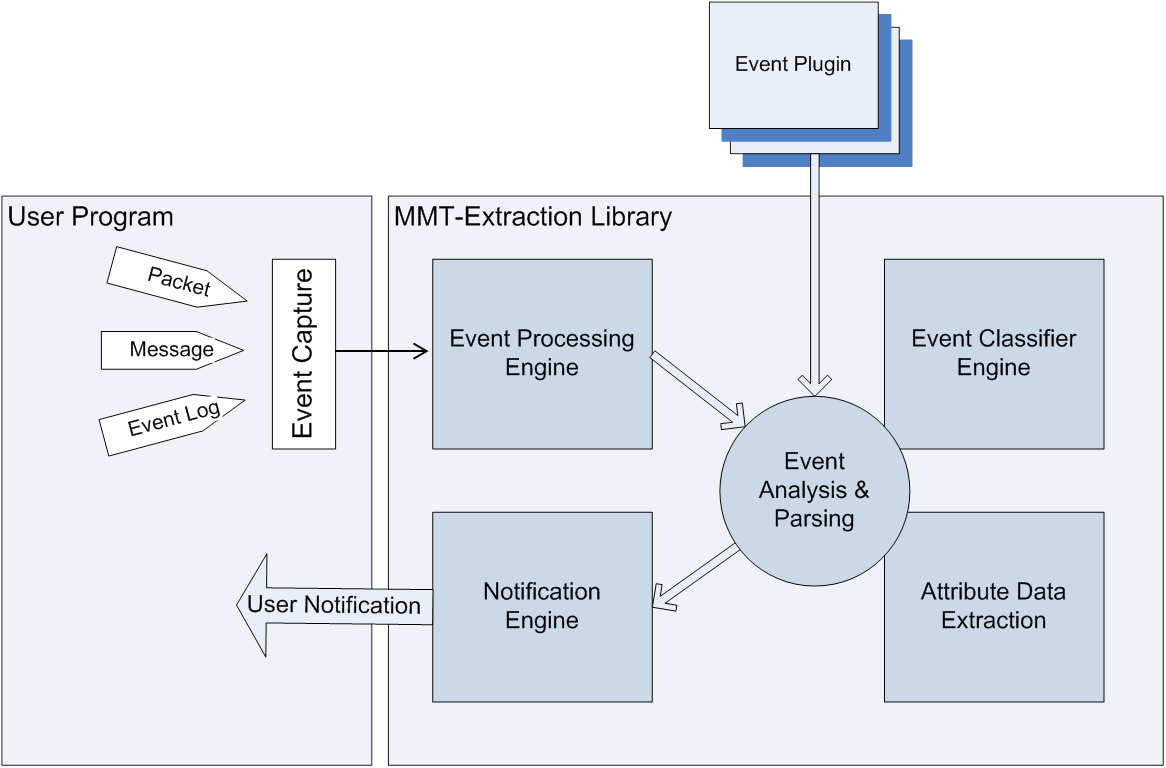
\includegraphics[width=4in]{img/extract_lib.png}
\caption{MMT-DPI Library}\label{extract_lib}
\end{figure}


\subsubsection{Using MMT-DPI in a development project}
In order to use the MMT-DPI library in a development project, one must perform the followings:

\begin{itemize}
\item Include the header file \path{mmt_core.h}: This file is the only one that needs to be included. 
\item By default, the plugins folder locates at \path{/opt/mmt/plugins} after installing MMT-DPI. However you can create a folder called \path{plugins} in the directory where the executable is located, then you should copy the file \path{libmmt_tcpip.so} into \path{plugins} to be able to analyse TCP/IP based network traffic. If one has developped any new MMT-DPI plugin, it must be copied to this \path{plugins} folder. 
Explaining how to add new plugins is described later in this document;
\item Build a \path{main.c} program that uses the library's API (see the following section);
\item Compile the program, linking the MMT-DPI library by using the option: \path{-I/opt/mmt/dpi/include} \path{-L/opt/mmt/dpi/lib} \path{-lmmt_core}
\end{itemize}
\subsubsection{Extraction API description }
The MMT-DPI API is specified in the header files provided with the download package. In the following we will shortly describe the content of the different header files:


\begin{itemize}
\item \path{mmt_core.h}: this is where the core extraction API functions are defined; 
\item \path{data_defs.h}: this is where the data related API functions are defined. In addition, the different data structures that might be used in an integration project are defined here;
\item \path{types_defs.h}: this is where the new data types are defined;
\item \path{extraction_lib.h}: this file contains the generic extraction functions;
\item \path{plugin_defs.h}: this file contains the definitions that can be used for the plugin development.
\end{itemize}

\index{initialization}\marginlabel{Initialization:}
In order to use the MMT-DPI library, one must initialize it by using the following function signature:

\begin{lstlisting}[style=Cpp]
init_extraction () ;
\end{lstlisting}

The initialization returns a positive number on success and zero on failure. It is good practice to always check the return number of \inlineCode{init\_extraction()}.

The following function will create an extraction handler:

\begin{lstlisting}[style=Cpp]
mmt_handler_t *mmt = mmt_init_handler (
        uint32_t stacktype,
        uint32_t options,
        char     *errbuf );
\end{lstlisting}

where the \inlineCode{stacktype} is 1 for 10Mb Ethernet, \inlineCode{options} is 0 and \inlineCode{errbuf} is a \inlineCode{char [1024]} to hold any error message in the case that the return value is \inlineCode{NULL}. The return value is the handle and will be needed by the other functions that need to be called.

For capturing the packets, you can select any library such as: DPDK, PCAP,... In some of our example, we use the PCAP library and, in particular, the following functions (not detailed in this document):
\begin{itemize}
\item    \inlineCode{pcap\_open\_live}
\item    \inlineCode{pcap\_open\_offline}
\item    \inlineCode{pcap\_next}
\item    \inlineCode{pcap\_loop}
\item    \inlineCode{pcap\_close}
\end{itemize}    
    
Each time a packet is recuperated using \inlineCode{pcap\_next} or \inlineCode{pcap\_loop}, it is passed over to the Event Processing Engine using the \inlineCode{packet\_process} function described below in Message processing.

The following function will close the extraction handler and free any previously allocated memory:

\begin{lstlisting}[style=Cpp]
void mmt_close_handler( mmt_handler_t * mmt );
\end{lstlisting}

The following function will close the extraction and free any previously allocated memory:

\begin{lstlisting}[style=Cpp]
int close_extraction ();
\end{lstlisting}

\index{processing}\marginlabel{Message processing:}
MMT-DPI can process network packets in the de-facto PCAP\footnote{PCAP reference} format, raw messages, log messages, etc. 

The following function hands a packet to the core engine of MMT-DPI:

\begin{lstlisting}[style=Cpp]
int packet_process (
    mmt_handler_t *mmt,
    struct pkthdr *header,
    u_char        *packet );
\end{lstlisting}

This function should be called for every packet to process. The \inlineCode{header} parameter of the function is a pointer to the meta-data of the message that include the message arrival time, the message length, etc. The \inlineCode{packet} parameter of the function is a pointer to the message data. The \inlineCode{packet\_process} function will return a positive value on successful processing. Zero is returned if an internal error is encountered, although this should never happen.

\index{registring}\marginlabel{Registering extraction attributes:}
The MMT-DPI library allows registering attributes for extraction. This limits the extraction overhead since only the data that is needed is recuperated. Attributes are fields in a network packet, specific data in a log entry, etc. 


The any of the following two functions can be used to register an attribute for extraction:

\begin{lstlisting}[style=Cpp]
void register_extraction_attribute (
    mmt_handler_t *mmt,
    uint32_t       protocol_id, 
    uint32_t       attribute_id );
\end{lstlisting}

\begin{lstlisting}[style=Cpp]
void register_extraction_attribute_by_name (
    mmt_handler_t *mmt,
    const char    *proto_name,
    const char    *attribute_name);
\end{lstlisting}

An attribute is identified by the protocol and attribute id or names. If the registration succeeds, a positive value will be returned; zero is returned on failure.

The following function allows verifying if an attribute, identified by its protocol and attribute identifiers, is already registered:

\begin{lstlisting}[style=Cpp]
int is_registered_attribute (
        mmt_handler_t *mmt,
        uint32_t       protocol_id,
        uint32_t       attribute_id );
\end{lstlisting}

This function will return a positive value if the attribute is already registered.


The any of the two following functions allow unregistering an attribute:

\begin{lstlisting}[style=Cpp]
int unregister_extraction_attribute (
    mmt_handler_t *mmt,
    uint32_t       protocol_id,
    uint32_t       attribute_id );
\end{lstlisting}

\begin{lstlisting}[style=Cpp]
int unregister_extraction_attribute_by_name (
    mmt_handler_t *mmt,
    uint32_t       proto_name,
    uint32_t       attribute_name );
\end{lstlisting}

If the unregistration succeeds, a positive value will be returned.

To recuperate the data in an attribute, any of the following two functions will return a pointer to the data if it was detected in the current event (i.e., the current packet that is being analysed). If the attribute or data does not exist for the current event then \inlineCode{NULL} will be returned.

\begin{lstlisting}[style=Cpp]
void * get_attribute_extracted_data (
    mmt_handler_t *mmt,
    uint32_t       protocol_id,
    uint32_t       attribute_id);
\end{lstlisting}

\begin{lstlisting}[style=Cpp]
void * get_attribute_extracted_data_by_name (
    mmt_handler_t *mmt,
    const char    *protocol_name,
    const char    *attribute_name );
\end{lstlisting} 

\index{callbacks}\marginlabel{Registering callbacks:}
The MMT-DPI library allows registering callback functions. A registered callback function will be called following the extraction of attributes whenever a packet is processed. 


The following function allows registering a packet handler:

\begin{lstlisting}[style=Cpp]
int register_packet_handler (
    mmt_handler_t                  *mmt,
    int                             handler_id,
    generic_packet_handler_callback function,
    u_char                         *args );
\end{lstlisting}

A packet handler is a callback that will be called each time a packet is processed. If needed, the user can provide a pointer to an argument that will be passed to the callback function when it is called. The callback function is associated with an identifier that should be unique, i.e., two callback functions cannot have the same identifier. This function will return a positive value upon success.

To verify that a packet handler callback function is registered with a given identifier, one can use the following function:

\begin{lstlisting}[style=Cpp]
int is_registered_packet_handler (
        mmt_handler_t  *mmt,
        int             handler_id );
\end{lstlisting}




This function returns a positive value if a registered callback function is found for the provided identifier.




In order to unregister an already registered packet handler one can use:




\begin{lstlisting}[style=Cpp]
int unregister_packet_handler (
        mmt_handler_t *mmt,
        int            handler_id );
\end{lstlisting}




In addition to packet handlers, it is possible to register a callback function to be called when an attribute is detected. This can be done with the following function:




\begin{lstlisting}[style=Cpp]
int register_attribute_handler (
        mmt_handler_t             *mmt,
        uint32_t                   protocol_id,
        uint32_t                   attribute_id,
        attribute_handler_function handler_fct,
        void                      *handler_condition,
        void                      *user_args );
\end{lstlisting}




This function allows registering an attribute handler that is a callback that will be called when the attribute defined by the given protocol and attribute ids is detected (i.e, not NULL). If needed, the user can provide a pointer to an argument that will be passed to the callback function when it is called. In the current version the parameter defined by \inlineCode{handler\_condition} is not implemented and should be set to NULL. This function will return a positive value upon success.


The following function registers an attribute handler given by its protocol and attribute names:


\begin{lstlisting}[style=Cpp]
int register_attribute_handler_by_name (
        mmt_handler_t *mmt,
        const char    *protocol_name,
        const char    *attribute_name,
        attribute_handler_function handler_fct,
        void *handler_condition,
        void *user_args);
\end{lstlisting}

To verify that an attribute handler is registered, one can use the following function:

\begin{lstlisting}[style=Cpp]
int has_registered_attribute_handler (
        mmt_handler_t *mmt,
        uint32_t       protocol_id,
        uint32_t       attribute_id );
\end{lstlisting}

This function returns a positive value if a handler is already registered with the attribute defined by its protocol and attribute identifiers.

In order to unregister an already registered attribute handler one can use:

\begin{lstlisting}[style=Cpp]
int unregister_attribute_handler (
        mmt_handler_t * mmt,
        long protocol_id,
        long attribute_id );
\end{lstlisting}

\begin{lstlisting}[style=Cpp]
int unregister_attribute_handler_by_name (
        mmt_handler_t *mmt,
        const char    *protocol_name,
        const char    *attribute_name );
\end{lstlisting}


\index{functions}\marginlabel{Data functions:}
In addition to the core functions presented so far, MMT-DPI provides a number of utility functions to assist the user of the library. 

The following function returns the protocol name for a given numeric identifier:

\begin{lstlisting}[style=Cpp]
const char * get_protocol_name_by_id (
        mmt_handler_t *mmt,
        uint32_t       protocol_id );
\end{lstlisting}

NULL is returned if the given identifier does not correspond to any configured protocol. 


The following function returns the identifier of the protocol for a given name:

\begin{lstlisting}[style=Cpp]
long get_protocol_id_by_name (
        mmt_handler_t *mmt,
        const char    *protocol_name );
\end{lstlisting}

Zero is returned if the given name does not correspond to any configured protocol. 


The following function indicates if the attribute exists for given protocol and attribute ids.


\begin{lstlisting}[style=Cpp]
int is_protocol_attribute (
        mmt_handler_t *mmt,
        uint32_t       protocol_id,
        uint32_t       attribute_id );
\end{lstlisting}



The following function returns the name of the attribute corresponding to the given protocol and attribute identifiers:

\begin{lstlisting}[style=Cpp]
const char * get_attribute_name_by_protocol_and_attribute_ids (
        mmt_handler_t *mmt,
        uint32_t       protocol_id,
        uint32_t       attribute_id );
\end{lstlisting}

NULL is returned if there is no attribute corresponding to the given identifiers. 


The following function returns the identifier of the attribute corresponding to the given protocol and attribute names:

\begin{lstlisting}[style=Cpp]
long get_attribute_id_by_protocol_and_attribute_names (
        mmt_handler_t *mmt,
        const char    *protocol_name,
        const char    *attribute_name );
\end{lstlisting}

Zero is returned if there is no attribute corresponding to the given names. 


The following function returns the identifier of the attribute corresponding to the given protocol id and attribute name:

\begin{lstlisting}[style=Cpp]
long get_attribute_id_by_protocol_id_and_attribute_name (
        mmt_handler_t *mmt,
        uint32_t       protocol_id,
        const char    *attribute_name );
\end{lstlisting}

Zero is returned if there is no attribute corresponding to the given parameters. 


The following function returns the identifier of the data type of the attribute corresponding to the given protocol and attribute identifiers:

\begin{lstlisting}[style=Cpp]
long get_attribute_data_type (
        mmt_handler_t *mmt,
        uint32_t       protocol_id,
        uint32_t       attribute_id );
\end{lstlisting}

Zero is returned if there is no attribute corresponding to the given parameters. 


The following function returns the data size, in number of bytes, of the attribute corresponding to the given protocol and attribute identifiers:

\begin{lstlisting}[style=Cpp]
int get_data_size_by_proto_and_field_ids (
        mmt_handler_t *mmt, 
        uint32_t       protocol_id, 
        uint32_t       attribute_id );
\end{lstlisting} 

Zero is returned if there is no attribute corresponding to the given parameters. 


The following function returns the data size of the given MMT data type:

\begin{lstlisting}[style=Cpp]
int get_data_size_by_data_type (
        mmt_handler_t *mmt,
        int            data_type );
\end{lstlisting}

Zero is returned if the data type is unknown.


The following function returns the position in the message of the attribute corresponding to the given protocol and attribute identifiers:

\begin{lstlisting}[style=Cpp]
int get_field_position_by_protocol_and_field_ids (
        mmt_handler_t *mmt,
        uint32_t       protocol_id,
        uint32_t       attribute_id );
\end{lstlisting}

For attributes where the position depends on the content of the message, \inlineCode{POSITION\_NOT\_KNOWN} (value -1) will be returned. The position is defined as the byte offset from the beginning of the packet.


%****************************************************

\subsection{Building the main}

To build a main that uses the MMT-DPI and MMT-Security libraries one should carefully study the \path{ARP_probe} example (Sec.~\ref{arp_example}). The main steps that need to be followed for building a \path{main.c} are:

\begin{enumerate}

\item Implement a callback function that will be called each time MMT-DPI parse successfully a packet. In this function, one need to retrieve value of protocol attributes from MMT-DPI and pass them to MMT-Security by calling function \inlineCode{mmt\_sec\_process}.

% \begin{lstlisting}[style=Cpp]
% int packet_handler( const ipacket_t *ipacket, void *args ) {
%     int i;
%     mmt_sec_handler_t *handler = (mmt_sec_handler_t *)args;
%     message_t *msg = create_message_t();	
    
%     msg->timestamp = mmt_sec_encode_timeval( &pkt->p_hdr->ts );
%     msg->counter   = pkt->packet_id;
    
%     //get a list of proto/attributes being used by mmt-security
%     for( i=0; i<proto_atts_count; i++ )
%     	dpi_message_set_data( pkt, proto_atts[i]->dpi_type, msg, proto_atts[i]->proto_id, proto_atts[i]->att_id );
    
%     //if there is no interested information => free the created msg
%     if( msg->elements_count == 0 )
%         free_message_t( msg );
%     else
%         //forward information to mmt-security
%     	mmt_sec_process( handler, msg ); 
    
%     return 0;
% }
% \end{lstlisting}

\item
Implement a callback function \inlineCode{mmt\_sec\_callback} that will be is called by MMT-Security each time a property is satisfied

% \begin{lstlisting}[style=Cpp]
% typedef void (*mmt_sec_callback)(
%   const rule_info_t *rule //rule being validated
%   enum verdict_type verdict, //DETECTED, NOT_RESPECTED
%   uint64_t timestamp, //moment (by time) the rule is validated
%   uint64_t counter,  //moment (by order of packet) the rule is validated
%   const mmt_array_t* const trace,//historic of messages that validates the rule
%   void *user_data //#user-data being given in mmt_sec_register_rules
% );
% \end{lstlisting}

\item
Call the functions that initialize the processing:

\begin{itemize}
    \item \inlineCode{init\_extraction}
    \item \inlineCode{mmt\_init\_handler}
    \item \inlineCode{mmt\_sec\_init}
    \item \inlineCode{mmt\_sec\_register}
\end{itemize}

\item
Initialise the PCAP API by calling one of the following functions:
\begin{itemize}
\item
\inlineCode{pcap\_open\_live}: for real time live analysis
\item
\inlineCode{pcap\_open\_offline}: for offline analysis
\end{itemize}

\item
Perform the loop that reads a packet from the input trace file or the network interface. This includes the following:\begin{itemize}
\item 
    Call the function: \inlineCode{pcap\_next}
\item 
    Set the header for the message before processing the packet:

\begin{itemize}
\item
        set timestamp:\newline 
        header.ts = p\_pkthdr.ts;
\item
        set length of data available for the packet:\newline 
        header.caplen = p\_pkthdr.caplen;
\item
        set length of packet:\newline     
        header.len = p\_pkthdr.len;
\item
        currently not used but should be set to NULL:\newline 
        header.user\_args = NULL;
\end{itemize}

\item 
    Call MMT-DPI lib function that will parse the packet and analyse it:
        \inlineCode{packet\_process}
        
    Note that each time a relevant packet (according to security properties) is received the \inlineCode{mmt\_sec\_process} function will be executed and, when a security property is satisfied or reaches a not satisfied condition, the callback function \inlineCode{mmt\_sec\_callback} will be executed.
\end{itemize}

\item
Call the functions that end the processing:

\begin{itemize}
   \item \inlineCode{mmt\_sec\_unregister}
   \item \inlineCode{mmt\_sec\_close}
   \item \inlineCode{mmt\_close\_handler}
   \item \inlineCode{pcap\_close}
\end{itemize}

\end{enumerate}


%****************************************************
\subsection{Add a new Protocol}

\subsubsection{MMT Plugin API}

The MMT-DPI library has a plugin architecture. It is possible to extend the extraction engine with new protocols. For this, a plugin needs to be created specifying the extraction to add. An MMT plugin will initialize a protocol structure that contains the required information regarding the protocol attributes, as well as the functions allowing extracting the data corresponding to these attributes. In this section we will describe the required steps in order to create a new MMT plugin.

When creating a new MMT plugin, you must use the API functions described in the following sub-sections.

\marginlabel{Initializing a protocol structure}
Creating a new plugin requires the initialization of a protocol structure. A protocol is defined by a unique identifier. The first step in the process of creating a plugin is to get a protocol structure using the following function:

\begin{lstlisting}[style=Cpp]
protocol_t *init_protocol_struct_for_registration (
        int         protocol_id, 
        const char *protocol_name);
\end{lstlisting}

This function will return a pointer to a free protocol structure with the given identifier. If a protocol with the same identifier is already registered, this function will return NULL.

\marginlabel{Registering protocol attributes}
Once the protocol structure is initialized, you need to add the attributes belonging to the protocol. An attribute has an identifier, a name, a data type, a data length, a position within the packet (offset), a scope (packet or session) and an extraction function (can be generic if the position and data length are known). 

\begin{lstlisting}[style=Cpp]
int register_attribute_with_protocol (
        protocol_t          *protocol_struct, 
        attribute_metadata_t attr);
\end{lstlisting}                                                

This function registers the attribute \inlineCode{attr} with the protocol \inlineCode{protocol\_struct}. 

\marginlabel{Registering a classification function with parent protocol}
For some protocol which is encapsulated in other protocols (parent protocols), you need to register a classification function with parent protocols to. For example, the classification function of "HTTP" protocol need to register with parent protocol is \inlineCode{TCP}. The classification function is protocol specific and needs to be implemented by the user. 

\begin{lstlisting}[style=Cpp]
void register_classification_function_with_parent_protocol (
        uint32_t                        parent_protocol_id, 
        generic_classification_function classification_fct, 
        int                             weight);
\end{lstlisting}  

This function registers a classification function \inlineCode{classification\_fct} with the parent protocol is the given \inlineCode{parent\_protocol\_id}.

\marginlabel{Registering a classification function (optional)}
Once the protocol structure is initialized, you need to add a classification function. A classification function identifies the type of protocol/message encapsulated in the current protocol/message. For example, the classification function of \inlineCode{IP} protocol will tell if the encapsulated protocol is \inlineCode{TCP}, \inlineCode{UDP}, \inlineCode{ICMP}, etc. The classification function is protocol specific and needs to be implemented by the user. 

\begin{lstlisting}[style=Cpp]
void register_classification_function (
        protocol_t                     *protocol_struct, 
        generic_classification_function classification_fct);
\end{lstlisting}  

This function registers a classification function \inlineCode{classification\_fct} for the protocol identified by the \inlineCode{protocol\_struct} parameter. The signature of the classification function is defined by the function type \inlineCode{generic\_classification\_function} defined in \inlineCode{mmt\_core.h}

\marginlabel{Registering an initialized protocol structure}
The final step when creating a plugin is to register the created protocol structure in the MMT-DPI. For this purpose, you must use the following function:

\begin{lstlisting}[style=Cpp]
int register_protocol (
        protocol_t *protocol_struct, 
        uint32_t    protocol_id);
\end{lstlisting}

This function registers the protocol defined by the given protocol structure and protocol identifier in the extraction core. Remember that a protocol has a unique identifier, and registering a protocol structure with an already used identifier will cause the function to fail. On success, this function will return \inlineCode{PROTO\_REGISTERED} (value 1). \inlineCode{PROTO\_NOT\_REGISTERED} (value 0) will be 
returned on failure.

\marginlabel{Utility functions}
The MMT Plugin API has a number of utility functions that can be very useful when creating a new plugin. 

\begin{lstlisting}[style=Cpp]
int is_valid_protocol_id ( uint32_t protocol_id );
\end{lstlisting}

This function verifies if a given identifier is valid. A protocol identifier must have a positive value less than the \inlineCode{PROTO\_MAX\_IDENTIFIER}. A positive value is returned if the given identifier is valid, a negative value otherwise.

\begin{lstlisting}[style=Cpp]
int is_registered_protocol ( uint32_t protocol_id );
\end{lstlisting}

This function verifies if a protocol with the given identifier is already registered. \inlineCode{PROTO\_REGISTERED} (value 1) is returned if a protocol is already registered, \inlineCode{PROTO\_NOT\_REGISTERED} (value 0) is returned otherwise.

\begin{lstlisting}[style=Cpp]
int is_free_protocol_id_for_registraction ( 
        uint32_t protocol_id );
\end{lstlisting}

This function returns a positive value if there is no protocol registered with the given identifier. A negative value is returned otherwise.

\marginlabel{Generic extraction functions}
A number of generic extraction functions are implemented in the MMT-DPI and can be reused by the plugins. They include:

\begin{lstlisting}[style=Cpp]
int general_byte_to_byte_extraction (
        const ipacket_t *packet, 
        int              proto_index, 
        attribute_t     *extracted_data);
\end{lstlisting}

This is a generic extraction function. It will copy, into the data part of \inlineCode{extracted\_data} structure a defined number of bytes from the data part of the packet structure. Any extraction function must have the same signature and must return a positive value if the extraction is successful.

\begin{lstlisting}[style=Cpp]
int general_short_extraction_with_ordering_change(
        const ipacket_t *packet, 
        int              proto_index, 
        attribute_t     *extracted_data);

int general_int_extraction_with_ordering_change(
        const ipacket_t *packet, 
        int              proto_index, 
        attribute_t     *extracted_data);

int general_short_extraction(
        const ipacket_t *packet, 
        int              proto_index, 
        attribute_t     *extracted_data);

int general_int_extraction(
        const ipacket_t *packet, 
        int              proto_index, 
        attribute_t     *extracted_data);
\end{lstlisting}

These 4 functions provide the extraction of \inlineCode{short} (2 bytes) and \inlineCode{int} (4 bytes) data with or without ordering change. 

\marginlabel{Utility structures}
In addition to the utility functions, the MMT Plugin API has a number of structures that can help organize plugin related data. 

\begin{lstlisting}[style=Cpp]
typedef struct attribute_metadata_struct {
  int id; /**< identifier of the attribute. */
  char alias[Max_Alias_Len + 1]; /**< the alias(name) of the attribute */
  int data_type; /**< the data type of the attribute */
  int data_len; /**< the data length of the attribute */
  int position_in_packet; /**< the position in the packet of the attribute. */
  int scope; /**< the scope of the attribute (packet, session, ...). */
  generic_attribute_extraction_function extraction_function; /**< the extraction function for this attribute. */
} attribute_metadata_t;
\end{lstlisting}

This structure defines the attribute related information; it can be used to model the information of the protocol attributes. 

This can be seen in the following code for the UDP protocol, that models UDP's attributes related information.  

\begin{lstlisting}[style=Cpp]
static attribute_metadata_t udp_attributes_metadata[UDP_ATTRIBUTES_NB] = {
  {UDP_SRC_PORT, UDP_SRC_PORT_ALIAS, MMT_U16_DATA, sizeof (short), 0, SCOPE_PACKET, general_short_extraction_with_ordering_change},
  {UDP_DEST_PORT, UDP_DEST_PORT_ALIAS, MMT_U16_DATA, sizeof (short), 2, SCOPE_PACKET, general_short_extraction_with_ordering_change},
  {UDP_LEN, UDP_LEN_ALIAS, MMT_U16_DATA, sizeof (short), 4, SCOPE_PACKET, general_short_extraction_with_ordering_change},
  {UDP_CHECKSUM, UDP_CHECKSUM_ALIAS, MMT_U16_DATA, sizeof (short), 6, SCOPE_PACKET, general_short_extraction_with_ordering_change},
};
\end{lstlisting}

\subsubsection{Create a MMT Plugin}

A MMT plugin, as described above, will initialize and register a protocol structure. This initialization/registration must be performed by using a function called \inlineCode{init\_proto}. When the Extraction core tries to load a plugin, it will search for and execute the function with this name. If the plugin does not implement such a function, it is considered invalid. Therefore, the creation of a new plugin is equivalent to the implementation of this function \inlineCode{init\_proto}. 
The following steps describe the creation of a plugin:

\marginlabel{Pre-step}
Create a new function \inlineCode{init\_proto}

\begin{lstlisting}[style=Cpp]
int init_proto();
\end{lstlisting}

This function must implement the next steps. It is highly recommended that you use the utility function when creating a plugin. 
First step

Request a protocol structure with a defined protocol identifier for initialization using: 
\begin{lstlisting}[style=Cpp]
protocol_t *init_protocol_struct_for_registration(
    uint32_t    protocol_id, 
    const char *protocol_name);
\end{lstlisting}

\marginlabel{Second step}
Define the protocol attributes and create an array of the attributes. Register the defined attributes with the protocol structure initialized in step 1. 

This is where the protocol specific code will be created. 

\marginlabel{Third step}
If the current protocol is encapsulated in other protocols, you need to register a classification function with parent protocols. For example, the classification function of \inlineCode{QUIC} protocol need to register with parent protocol is \inlineCode{UDP} protocol. To register a classification function with parent protocol use:

\begin{lstlisting}[style=Cpp]
void register_classification_function_with_parent_protocol(
    uint32_t                        parent_protocol_id, 
    generic_classification_function classification_fct,
    int                             weight);
\end{lstlisting}

Of the protocol does not require a classification function from parent protocols (or it does not have any parent protocol), this step can be omitted. For example \inlineCode{ETHERNET} protocol does not have a parent protocols and thereforce it does not require registering a classifification with parent protocol.

\marginlabel{Forth step}
Once the protocol structure is initialized, you can add a classification function. A classification function identifies the type of protocol/message encapsulated in the current protocol/message. For example, the classification function of \inlineCode{IP} protocol will tell if the encapsulated protocol is \inlineCode{TCP}, \inlineCode{UDP}, \inlineCode{ICMP}, etc. The classification function is protocol specific and needs to be implemented by the user. To register a classification function use:

\begin{lstlisting}[style=Cpp]
void register_classification_function(
        protocol_t *protocol_struct, 
        generic_classification_function classification_fct);
\end{lstlisting}

If the protocol does not require a classification function, this step can be omitted, or NULL can be registered. For example, ARP protocol does not encapsulate any other protocol, and therefore it does not require a classification function.

\marginlabel{Fifth step}
The final step, when creating a plugin, is to register the created protocol structure in the MMT-Extraction core. For this purpose, you must use:

\begin{lstlisting}[style=Cpp]
int register_protocol(
        protocol_t *protocol_struct, 
        uint32_t    protocol_id);

\end{lstlisting}
This function will register the protocol structure if no other protocol is already registered with the given protocol identifier. 

If the protocol registration is successful, the plugin function \inlineCode{init\_proto} must return a positive value indicating that the plugin has been successfully loaded; otherwise a negative value must be returned to let the core perform the necessary cleanup. 

\subsubsection{Create a MMT Plugin by using Plugin Generator}

You can create a MMT Plugin by using Plugin Generator. It is a Java Application which can create generate a basic source of a plugin bases on the plugin file

\marginlabel{Create plugin file}
The plugin file contains the basic information to generate a plugin. 

The ETHERNET protocol plugin can be created base on the following plugin file:

\begin{lstlisting}[style=Cpp]
Protocol {
  define ETH_P_IP = 0x0800
  define ETH_P_ARP = 0x0806
  define ETH_P_IPV6 = 0x86DD
  define ETH_P_RARP = 0x8035
  define PROTO_ARP = 11
  define PROTO_IP = 15
  define PROTO_IP6 = 16
  
  Properties {
    label = "ETHERNET"
    id = "12"
    context = "false"
    session = "false"
    encapsulation = "true"
    encoding = "network"
  }
  
  Attributes {
    struct ethhdr {
      MMT_DATA_MAC_ADDR h_dest;
      MMT_DATA_MAC_ADDR h_source;
      uint16_t h_proto;
    }
    attribute {
      alias="src" data_type="MMT_DATA_MAC_ADDR" data_len="sizeof (mac_addr_t)" 
      offset="0" scope="SCOPE_PACKET"
    }
    attribute {
      alias="dst" data_type="MMT_DATA_MAC_ADDR" data_len="sizeof (mac_addr_t)" 
      offset="2" scope="SCOPE_PACKET"
    }
  }
  
  classifynext {
    switch(val(h_proto)) {
      case ETH_P_IP: 
      nextencaps = PROTO_IP
      nextoffset = sizeof(struct ethhdr)
      break
      case ETH_P_ARP:
      nextencaps = PROTO_ARP
      nextoffset = sizeof(struct ethhdr)
      break
      case ETH_P_IPV6:
      nextencaps = PROTO_IP6
      nextoffset = sizeof(struct ethhdr)
      break
      case ETH_P_RARP:
      nextencaps = PROTO_ARP
      nextoffset = sizeof(struct ethhdr)
      break
      default:
      break
    }
  }
}
\end{lstlisting}

Another example about QUIC protocol:

\begin{lstlisting}[style=Cpp]
Protocol {
  Properties {
    label = "QUIC"
    id = "630"
    context = "false"
    session = "false"
    encapsulation = "false"
    encoding = "network"
  }
  Attributes {
    attribute {
      alias="connection_id" data_type="MMT_U32_DATA" data_len="sizeof(int)" 
      offset="0" scope="SCOPE_PACKET"
    }
    attribute {
      alias="sequence" data_type="MMT_U32_DATA" data_len="sizeof(int)" 
      offset="0" scope="SCOPE_PACKET"
    }
  }
}
\end{lstlisting}

In the plugin file, we can define the protocol properties: label, id, context, session (\true: if the protocol maintains session, \false: if the protocol does not maintain session), encapsulation (true: if the protocol encapsulates other protocol), encoding. We also can define the attributes of protocols: header structure, attribute extractions. Finally we can define the classification function of the protocol if it encapsulates other protocol.

\marginlabel{Generate basic plugin source code}
After creating the plugin file, we can generate the source code for new plugin by using the \inlineCode{MMTPluginGenerator} (please contact Montimage if you need this tool).

\begin{lstlisting}[style=BASH]
java -jar MMTPluginGenerator.jar plugin_file plugin_dir
\end{lstlisting}

There will be 2 source files generated, a \path{.c} file and a \path{.h} file.

For example, to generate source code for ETHERNET plugin:

\begin{lstlisting}[style=BASH]
mkdir quic_src
java -jar MMTPluginGenerator.jar quic quic_src/
ls quic_src/
quic_mmt_plugin.c quic_mmt_plugin.h
\end{lstlisting}

Following is the \path{quic_mmt_plugin.h} file generated by Plugin Generator

\begin{lstlisting}[style=Cpp]
/* Generated with MMT Plugin Generator */

#ifndef QUIC_H
#define QUIC_H
#ifdef  __cplusplus
extern "C" {
#endif

#include "plugin_defs.h"
#include "mmt_core.h"


#define PROTO_QUIC 630

#define PROTO_QUIC_ALIAS "QUIC"


enum quic_attributes {

  QUIC_CONNECTION_ID = 1,

  QUIC_SEQUENCE,

  QUIC_ATTRIBUTES_NB = QUIC_SEQUENCE,

};


#define QUIC_CONNECTION_ID_ALIAS "connection_id"

#define QUIC_SEQUENCE_ALIAS "sequence"


int init_quic_proto_struct();



#ifndef CORE
int init_proto();
#endif //CORE



#ifdef  __cplusplus
}
#endif
#endif  /* QUIC_H */

\end{lstlisting}

Following is the \path{quic_mmt_plugin.c} file generated by Plugin Generator

\begin{lstlisting}[style=Cpp]
/* Generated with MMT Plugin Generator */

#include <stdio.h>
#include <stdlib.h>
#include <string.h>
#include "quic_mmt_plugin.h"
#include "extraction_lib.h"




/*
 * QUIC data extraction routines
 */



int quic_connection_id_extraction(const ipacket_t * ipacket, int proto_index,
                                  attribute_t * extracted_data) {
  /* Get the protocol offset */
  int proto_offset = get_packet_offset_at_index(ipacket, proto_index);


  int attribute_offset = quic_attributes_metadata[0].position_in_packet;


  /* Get the attribute data length */
  int attribute_length = sizeof(MMT_U32_DATA);


  *((unsigned int *) extracted_data->data) = ntohl(*((unsigned int *) & ipacket->data[proto_offset + attribute_offset]));



  return 1;
}



int quic_sequence_extraction(const ipacket_t * ipacket, int proto_index,
                             attribute_t * extracted_data) {
  /* Get the protocol offset */
  int proto_offset = get_packet_offset_at_index(ipacket, proto_index);


  int attribute_offset = quic_attributes_metadata[1].position_in_packet;


  /* Get the attribute data length */
  int attribute_length = sizeof(MMT_U32_DATA);


  *((unsigned int *) extracted_data->data) = ntohl(*((unsigned int *) & ipacket->data[proto_offset + attribute_offset]));



  return 1;
}


classified_proto_t quic_stack_classification(ipacket_t * ipacket) {
  classified_proto_t retval;
  retval.offset = 0;
  retval.proto_id = PROTO_QUIC;
  retval.status = Classified;
  return retval;
}

static attribute_metadata_t quic_attributes_metadata[QUIC_ATTRIBUTES_NB] = {

  {QUIC_CONNECTION_ID, QUIC_CONNECTION_ID_ALIAS, MMT_U32_DATA, sizeof(uint32_t), 0, SCOPE_PACKET, quic_connection_id_extraction},

  {QUIC_SEQUENCE, QUIC_SEQUENCE_ALIAS, MMT_U32_DATA, sizeof(uint32_t), 0, SCOPE_PACKET, quic_sequence_extraction},

};


int init_quic_proto_struct() {
  protocol_t * protocol_struct = init_protocol_struct_for_registration(PROTO_QUIC, PROTO_QUIC_ALIAS);

  if (protocol_struct != NULL) {

    int i = 0;
    for (; i < QUIC_ATTRIBUTES_NB; i ++) {
      register_attribute_with_protocol(protocol_struct, &quic_attributes_metadata[i]);
    }


    register_protocol_stack(PROTO_QUIC, PROTO_QUIC_ALIAS, quic_stack_classification);
    return register_protocol(protocol_struct, PROTO_QUIC);
  } else {
    return -1;
  }
}

#ifndef CORE
int init_proto() {
  return init_quic_proto_struct();
}
#endif //CORE



\end{lstlisting}


From the basic source code, we need to complete the plugin by adding/updating some more function such as: classification functions, extraction functions,....

\marginlabel{Complete plugin\\source code:}
\textit{Register classification function with parent protocol}

After having the basic source code, we need to adding the classification functions if needed.

The following is the classification function of QUIC protocol which will be called in QUIC's parent protocol is UDP protocol, it needs to be registered with UDP protocol.

\begin{lstlisting}[style=Cpp]
int mmt_check_quic(ipacket_t * ipacket, unsigned index)
{
  printf("[inf] mmt_check_quic: %lu - %d\n", ipacket->packet_id, index );
  int l4_offset = get_packet_offset_at_index(ipacket, index);
  // int l4_packet_len = ipacket->p_hdr->caplen - l4_offset;
  struct udphdr * udp = NULL;
  udp = (struct udphdr *) & ipacket->data[l4_offset];
  char * payload = (char*) &ipacket->data[l4_offset + sizeof(struct udphdr)];
  int quic_offset = l4_offset + sizeof(struct udphdr);
  classified_proto_t quic_proto = quic_stack_classification(ipacket);
  quic_proto.offset = quic_offset;
  int ver_offs;
  if (udp != NULL) {
    uint16_t sport = ntohs(udp->source), dport = ntohs(udp->dest);
    // debug("QUIC: Calculating QUIC over UDP");
    if ((((sport == 80) || (dport == 80) || (sport == 443) || (dport == 443))))
    {
      // Settings without version. First check if PUBLIC FLAGS & SEQ bytes are 0x0. SEQ must be 1 at least.
      if ((payload[0] == 0x00 && payload[1] != 0x00) || ((payload[0] & QUIC_NO_V_RES_RSV) == 0))
      {
        int seq = sequence(payload);
        fprintf(stderr, "[PROTO_QUIC] %lu sequence: %d!\n", ipacket->packet_id, seq);
        if (seq < 1)
        {
          fprintf(stderr, "[PROTO_QUIC] %lu mmt_check_quic: Not QUIC!\n", ipacket->packet_id);
        }

        fprintf(stderr, "[PROTO_QUIC] %lu mmt_check_quic: FOUND QUIC!\n", ipacket->packet_id);
        return set_classified_proto(ipacket, index + 1, quic_proto);
      }

      // Check if version, than the CID length.
      else if (payload[0] & QUIC_VER_MASK)
      {
        // Skip CID length.
        ver_offs = connect_id(payload[0]);
        fprintf(stderr, "[PROTO_QUIC] %lu connection id: %d!\n", ipacket->packet_id, ver_offs);
        if (ver_offs >= 0)
        {
          unsigned char vers[] = {payload[ver_offs], payload[ver_offs + 1],
                                  payload[ver_offs + 2], payload[ver_offs + 3]
                                 };

          // Version Match.
          if ((vers[0] == 'Q' && vers[1] == '0') &&
              ((vers[2] == '2' && (vers[3] == '5' || vers[3] == '4' || vers[3] == '3' || vers[3] == '2' ||
                                   vers[3] == '1' || vers[3] == '0')) ||
               (vers[2] == '1' && (vers[3] == '9' || vers[3] == '8' || vers[3] == '7' || vers[3] == '6' ||
                                   vers[3] == '5' || vers[3] == '4' || vers[3] == '3' || vers[3] == '2' ||
                                   vers[3] == '1' || vers[3] == '0')) ||
               (vers[2] == '0' && vers[3] == '9')))

          {
            fprintf(stderr, "[PROTO_QUIC] %lu mmt_check_quic: FOUND QUIC!\n", ipacket->packet_id);
            return set_classified_proto(ipacket, index + 1, quic_proto);
          }
        }
      }
    }
    else
    {
      fprintf(stderr, "[PROTO_QUIC] %lu mmt_check_quic: Not QUIC!\n", ipacket->packet_id);
    }
  }
  fprintf(stderr, "[PROTO_QUIC] %lu mmt_check_quic: Not QUIC!\n", ipacket->packet_id);
  return 0;
}
\end{lstlisting}

The registering classification function with parent protocol is done in \inlineCode{init\_quic\_proto\_struct}:

\begin{lstlisting}[style=Cpp]
int init_quic_proto_struct() {
    protocol_t * protocol_struct = init_protocol_struct_for_registration(PROTO_QUIC, PROTO_QUIC_ALIAS);

    if (protocol_struct != NULL) {

        int i = 0;
        for(; i < QUIC_ATTRIBUTES_NB; i ++) {
            register_attribute_with_protocol(protocol_struct, &quic_attributes_metadata[i]);
        }

        if(!register_classification_function_with_parent_protocol(PROTO_UDP, mmt_check_quic, 50)){
            };
        return register_protocol(protocol_struct, PROTO_QUIC);
    } else {
        return -1;
    }
}
\end{lstlisting}

After the registration, the QUIC protocol plugin has been registered as a child protocol of UDP, and for any UDP packet, MMT-DPI will check whether it contains QUIC protocol.

\textit{Register classification function to find the next protocol}

If the current protocol encapsulates other protocol, then we need to register a classification function to find the next protocol. For example, following is the classification function to find the next protocol after ETHERNET protocol:

\begin{lstlisting}[style=Cpp]
int ethernet_classify_next_proto(ipacket_t * ipacket, unsigned index) {
    int offset = get_packet_offset_at_index(ipacket, index);

    const struct ethhdr *ethernet = (struct ethhdr *) & ipacket->data[offset];
    classified_proto_t retval;
    retval.offset = -1;
    retval.proto_id = -1;
    retval.status = NonClassified;
    switch (ntohs(ethernet->h_proto)) // Layer 3 protocol identifier
    {
            /* IPv4 */
        case ETH_P_IP:
            retval.proto_id = PROTO_IP;
            retval.offset = sizeof (struct ethhdr);
            retval.status = Classified;
            break;
            /* IPv6 */
        case ETH_P_IPV6:
            retval.proto_id = PROTO_IPV6;
            retval.offset = sizeof (struct ethhdr);
            retval.status = Classified;
            break;
            /* ARP */
            /* RARP: will be processed as ARP */
        case ETH_P_RARP:
        case ETH_P_ARP:
            retval.proto_id = PROTO_ARP;
            retval.offset = sizeof (struct ethhdr);
            retval.status = Classified;
            break;
            /* 802.1Q */
        case ETH_P_8021Q:
            retval.proto_id = PROTO_8021Q;
            retval.offset = sizeof (struct ethhdr);
            retval.status = Classified;
            break;
        case ETH_P_NDN:
            retval.proto_id = PROTO_NDN;
            retval.offset = sizeof (struct ethhdr);
            retval.status = Classified;
            break;
        case 0x9100:
        case 0x9200:
        case 0x9300:
            retval.proto_id = PROTO_8021Q;
            retval.offset = sizeof (struct ethhdr) + 4;
            retval.status = Classified;
            break;
             /* PPPoE Discovery */
        case ETH_P_PPPoED:
            retval.proto_id = PROTO_PPPOE;
            retval.offset = sizeof (struct ethhdr);
            retval.status = Classified;
            break;
            /* PPPoE Session */
        case ETH_P_PPPoES:
            retval.proto_id = PROTO_PPPOE;
            retval.offset = sizeof (struct ethhdr);
            retval.status = Classified;
            break;
            /* Batman */
        case ETH_P_BATMAN:
            retval.proto_id = PROTO_BATMAN;
            retval.offset = sizeof (struct ethhdr);
            retval.status = Classified;
            break;
            break;
            break;
        default:
            break;
    }
    return set_classified_proto(ipacket, index + 1, retval);
    //return retval;
}
\end{lstlisting}

The registration need to be done in \inlineCode{init\_proto\_ethernet\_struct}:

\begin{lstlisting}[style=Cpp]
int init_proto_ethernet_struct() {
    protocol_t * protocol_struct = init_protocol_struct_for_registration(PROTO_ETHERNET, PROTO_ETHERNET_ALIAS);

    if (protocol_struct != NULL) {

        int i = 0;
        for(; i < ETHERNET_ATTRIBUTES_NB; i ++) {
            register_attribute_with_protocol(protocol_struct, &ethernet_attributes_metadata[i]);
        }

        register_classification_function(protocol_struct, ethernet_classify_next_proto);

        // Ethernet is a major encapsulating protocol, register it as a stack
        register_protocol_stack(DLT_EN10MB, PROTO_ETHERNET_ALIAS, ethernet_stack_classification); //TODO: check the return value of this
        //register_protocol_stack_full(DLT_EN10MB, PROTO_ETHERNET_ALIAS, ethernet_stack_classification, ehternet_stack_internal_cleanup, (void *) setup_tcpip_internal_packet(), (void *) setup_tcpip_internal_context()); //TODO: check the return value of this

        return register_protocol(protocol_struct, PROTO_ETHERNET);
    } else {
        return 0;
    }
}
\end{lstlisting}

\textit{Complete the extracting functions}

For some attributes which cannot be extracted by generic function, we need to add/update the extrating functions. The following functions are the completed extracting function for QUIC protocol:

\begin{lstlisting}[style=Cpp]
int mmt_connection_id_extraction(const ipacket_t * ipacket, unsigned proto_index,
        attribute_t * extracted_data) {
        int l4_offset = get_packet_offset_at_index(ipacket, proto_index);
        char * payload =(char*) &ipacket->data[l4_offset + sizeof(struct udphdr)];
        int conn_id = connect_id(payload[0]);
        *((uint32_t *) extracted_data->data) = conn_id;
        return 1;
    }

int mmt_sequence_extraction(const ipacket_t * ipacket, unsigned proto_index,
        attribute_t * extracted_data) {
        int l4_offset = get_packet_offset_at_index(ipacket, proto_index);
        char * payload =(char*) &ipacket->data[l4_offset + sizeof(struct udphdr)];
        int seq = sequence(payload);
        *((uint32_t *) extracted_data->data) = seq;
        return 1;
    }
\end{lstlisting}

\textit{Other functions, variables, and macros...}

We also need to add some more functions, variables, and macros if needed.

The following source code is a completed source code for QUIC protocol:

\begin{lstlisting}[style=Cpp]
/* Generated with MMT Plugin Generator */

#include <stdio.h>
#include <stdlib.h>
#include <string.h>
#include "quic_mmt_plugin.h"
#include "extraction_lib.h"
#include "tcpip/mmt_tcpip.h"
#include <netinet/udp.h>


#define QUIC_NO_V_RES_RSV 0xC3  // 1100 0011

#define QUIC_CID_MASK 0x0C      // 0000 1100
#define QUIC_VER_MASK 0x01      // 0000 0001
#define QUIC_SEQ_MASK 0x30      // 0011 0000

#define CID_LEN_8 0x0C          // 0000 1100
#define CID_LEN_4 0x08          // 0000 1000
#define CID_LEN_1 0x04          // 0000 0100
#define CID_LEN_0 0x00          // 0000 0000

#define SEQ_LEN_6 0x30          // 0011 0000
#define SEQ_LEN_4 0x20          // 0010 0000
#define SEQ_LEN_2 0x10          // 0001 0000
#define SEQ_LEN_1 0x00          // 0000 0000

#define SEQ_CONV(ARR) (ARR[0] | ARR[1] | ARR[2] | ARR[3] | ARR[4] | ARR[5] << 8)


classified_proto_t quic_stack_classification(ipacket_t * ipacket) {
  classified_proto_t retval;
  retval.offset = 0;
  retval.proto_id = PROTO_QUIC;
  retval.status = Classified;
  return retval;
}


static int connect_id(char pflags)
{
  u_int cid_len;

  // Check CID length.
  switch (pflags & QUIC_CID_MASK)
  {
  case CID_LEN_8: cid_len = 8; break;
  case CID_LEN_4: cid_len = 4; break;
  case CID_LEN_1: cid_len = 1; break;
  case CID_LEN_0: cid_len = 0; break;
  default:
    return -1;

  }
  // Return offset.
  return cid_len + 1;
}

static int sequence(char *payload)
{
  unsigned char conv[6] = {0};
  u_int seq_value = -1;
  int seq_lens;
  int cid_offs;
  int i;

  // Search SEQ bytes length.
  switch (payload[0] & QUIC_SEQ_MASK)
  {
  case SEQ_LEN_6: seq_lens = 6; break;
  case SEQ_LEN_4: seq_lens = 4; break;
  case SEQ_LEN_2: seq_lens = 2; break;
  case SEQ_LEN_1: seq_lens = 1; break;
  default:
    return -1;
  }
  // Retrieve SEQ offset.
  cid_offs = connect_id(payload[0]);

  if (cid_offs >= 0 && seq_lens > 0)
  {
    for (i = 0; i < seq_lens; i++)
      conv[i] = payload[cid_offs + i];

    seq_value = SEQ_CONV(conv);
  }

  // Return SEQ dec value;
  return seq_value;
}

int mmt_check_quic(ipacket_t * ipacket, unsigned index)
{
  printf("[inf] mmt_check_quic: %lu - %d\n", ipacket->packet_id, index );
  int l4_offset = get_packet_offset_at_index(ipacket, index);
  // int l4_packet_len = ipacket->p_hdr->caplen - l4_offset;
  struct udphdr * udp = NULL;
  udp = (struct udphdr *) & ipacket->data[l4_offset];
  char * payload = (char*) &ipacket->data[l4_offset + sizeof(struct udphdr)];
  int quic_offset = l4_offset + sizeof(struct udphdr);
  classified_proto_t quic_proto = quic_stack_classification(ipacket);
  quic_proto.offset = quic_offset;
  int ver_offs;
  if (udp != NULL) {
    uint16_t sport = ntohs(udp->source), dport = ntohs(udp->dest);
    // debug("QUIC: Calculating QUIC over UDP");
    if ((((sport == 80) || (dport == 80) || (sport == 443) || (dport == 443))))
    {
      // Settings without version. First check if PUBLIC FLAGS & SEQ bytes are 0x0. SEQ must be 1 at least.
      if ((payload[0] == 0x00 && payload[1] != 0x00) || ((payload[0] & QUIC_NO_V_RES_RSV) == 0))
      {
        int seq = sequence(payload);
        fprintf(stderr, "[PROTO_QUIC] %lu sequence: %d!\n", ipacket->packet_id, seq);
        if (seq < 1)
        {
          fprintf(stderr, "[PROTO_QUIC] %lu mmt_check_quic: Not QUIC!\n", ipacket->packet_id);
        }

        fprintf(stderr, "[PROTO_QUIC] %lu mmt_check_quic: FOUND QUIC!\n", ipacket->packet_id);
        return set_classified_proto(ipacket, index + 1, quic_proto);
      }

      // Check if version, than the CID length.
      else if (payload[0] & QUIC_VER_MASK)
      {
        // Skip CID length.
        ver_offs = connect_id(payload[0]);
        fprintf(stderr, "[PROTO_QUIC] %lu connection id: %d!\n", ipacket->packet_id, ver_offs);
        if (ver_offs >= 0)
        {
          unsigned char vers[] = {payload[ver_offs], payload[ver_offs + 1],
                                  payload[ver_offs + 2], payload[ver_offs + 3]
                                 };

          // Version Match.
          if ((vers[0] == 'Q' && vers[1] == '0') &&
              ((vers[2] == '2' && (vers[3] == '5' || vers[3] == '4' || vers[3] == '3' || vers[3] == '2' ||
                                   vers[3] == '1' || vers[3] == '0')) ||
               (vers[2] == '1' && (vers[3] == '9' || vers[3] == '8' || vers[3] == '7' || vers[3] == '6' ||
                                   vers[3] == '5' || vers[3] == '4' || vers[3] == '3' || vers[3] == '2' ||
                                   vers[3] == '1' || vers[3] == '0')) ||
               (vers[2] == '0' && vers[3] == '9')))

          {
            fprintf(stderr, "[PROTO_QUIC] %lu mmt_check_quic: FOUND QUIC!\n", ipacket->packet_id);
            return set_classified_proto(ipacket, index + 1, quic_proto);
          }
        }
      }
    }
    else
    {
      fprintf(stderr, "[PROTO_QUIC] %lu mmt_check_quic: Not QUIC!\n", ipacket->packet_id);
    }
  }
  fprintf(stderr, "[PROTO_QUIC] %lu mmt_check_quic: Not QUIC!\n", ipacket->packet_id);
  return 0;
}



int mmt_connection_id_extraction(const ipacket_t * ipacket, unsigned proto_index,
                                 attribute_t * extracted_data) {
  int l4_offset = get_packet_offset_at_index(ipacket, proto_index);
  char * payload = (char*) &ipacket->data[l4_offset + sizeof(struct udphdr)];
  int conn_id = connect_id(payload[0]);
  *((uint32_t *) extracted_data->data) = conn_id;
  return 1;
}

int mmt_sequence_extraction(const ipacket_t * ipacket, unsigned proto_index,
                            attribute_t * extracted_data) {
  int l4_offset = get_packet_offset_at_index(ipacket, proto_index);
  char * payload = (char*) &ipacket->data[l4_offset + sizeof(struct udphdr)];
  int seq = sequence(payload);
  *((uint32_t *) extracted_data->data) = seq;
  return 1;
}

static attribute_metadata_t quic_attributes_metadata[QUIC_ATTRIBUTES_NB] = {

  {QUIC_CONNECTION_ID, QUIC_CONNECTION_ID_ALIAS, MMT_U32_DATA, sizeof(uint32_t), 0, SCOPE_PACKET, mmt_connection_id_extraction},

  {QUIC_SEQUENCE, QUIC_SEQUENCE_ALIAS, MMT_U32_DATA, sizeof(uint32_t), 0, SCOPE_PACKET, mmt_sequence_extraction},

};

int init_quic_proto_struct() {
  protocol_t * protocol_struct = init_protocol_struct_for_registration(PROTO_QUIC, PROTO_QUIC_ALIAS);

  if (protocol_struct != NULL) {

    int i = 0;
    for (; i < QUIC_ATTRIBUTES_NB; i ++) {
      register_attribute_with_protocol(protocol_struct, &quic_attributes_metadata[i]);
    }

    if (!register_classification_function_with_parent_protocol(PROTO_UDP, mmt_check_quic, 50)) {      
    };

    // register_protocol_stack(PROTO_QUIC, PROTO_QUIC_ALIAS, quic_stack_classification);
    return register_protocol(protocol_struct, PROTO_QUIC);
  } else {
    return -1;
  }
}

#ifndef CORE
int init_proto() {
  return init_quic_proto_struct();
}
#endif //CORE

\end{lstlisting}

After completing the source code, make sure you have installed MMT-DPI before compiling the plugin.

\subsubsection{Compile new plugin}

To compile new plugin, we can use the command line:

\begin{lstlisting}[style=BASH]
cd quic_src/
gcc -Wall -fPIC -shared -o libmmt_quic.so -I /opt/mmt/dpi/include/ quic_mmt_plugin.c
\end{lstlisting}

After executing the command, we should have the plugin file : \path{libmmt_quic.so}

\subsubsection{Install and test new plugin}

Now you have the plugin file (\path{.so} file), we are ready to install and test the new plugin.

\marginlabel{Install new plugin}
To install the plugin, simply copy the .so file into your plugins folder. (by default, the plugin folder locates in \path{/opt/mmt/plugins/})

\marginlabel{Test new plugin}
You can compile and run the file test \path{proto_attributes_iterator.c} (locates in \path{/opt/mmt/examples/}), if the plugin successfully installed, we should have something like this:

\begin{lstlisting}[style=Cpp]
$ ./proto_attributes_iterator
Protocol id 630 --- Name QUIC
    Attribute id 1 --- Name connection_id 
    Attribute id 2 --- Name sequence 
    Attribute id 4096 --- Name p_hdr 
    Attribute id 4097 --- Name p_data 
    Attribute id 4098 --- Name p_payload 
    Attribute id 4099 --- Name packet_count 
    Attribute id 4100 --- Name data_count 
    Attribute id 4101 --- Name payload_count 
    Attribute id 4102 --- Name ip_frag_packets_count 
    Attribute id 4103 --- Name ip_frag_data_volume 
    Attribute id 4104 --- Name ip_df_packets_count 
    Attribute id 4105 --- Name ip_df_data_volume 
    Attribute id 4106 --- Name session_count 
    Attribute id 4107 --- Name a_session_count 
    Attribute id 4108 --- Name t_session_count 
    Attribute id 4109 --- Name first_packet_time 
    Attribute id 4110 --- Name last_packet_time 
    Attribute id 4111 --- Name stats 
.. 
\end{lstlisting}

If you have the pcap file which contains the new protocol, you can compile and run the file \path{extract_all.c} (locates in \path{/opt/mmt/examples/}), the example will extract all attributes of all protocols.

\subsubsection{FAQ}

\textit{Question: Can we overwrite a plugin? }

\textit{Answer:} Yes and No

It totally depends on how we write the \inlineCode{init\_proto()} function.

If you don't want to overwrite plugin, you can check the return of the function \inlineCode{init\_quic\_proto\_struct()}. Otherwise you can ignore the return.

\textit{Not allow to overwrite:}

\begin{lstlisting}[style=Cpp]
/* quic_mmt_plugin.c - NOT OVERWRITE*/
#ifndef CORE
        int init_proto() {
            if (!init_quic2_proto_struct()) {
                exit(0);
            }
            return 1;
        }
#endif
\end{lstlisting}

\textit{Allow to overwrite:}

\begin{lstlisting}[style=Cpp]
/* quic_mmt_plugin.c - NOT OVERWRITE*/
#ifndef CORE
        int init_proto() {
            init_quic2_proto_struct();
        }
#endif
\end{lstlisting}


\textit{Question: Do we need to care about the order of plugins (.so files) in plugins/ folder?}

\textit{Answer:} Yes

The plugins will be loaded in alpha-beta order

The plugins should be loaded in dependency ordering

The overwrite plugin should be loaded after the old plugin

Independent plugin can be loaded without concern about the order

\textit{Best practice: Alway name your plugin after \path{libmmt_tcpip.so}}

%****************************************************


%%%%%%%%%%%%%%%%%%%%%%%%%%%%%%%%%%%%%%%%%%%%%%%%%%%%%%%%%%%%%%%%%%%%%%